\documentclass[12pt]{article}
\usepackage{amsmath}
\usepackage{amssymb}
\usepackage[letterpaper,top=1.2in,bottom=1in,left=0.75in,right=0.75in,centering]{geometry}
%\usepackage{fancyhdr}
\usepackage{enumerate}
%\usepackage{lastpage}
\usepackage{multicol}
\usepackage{graphicx}

\reversemarginpar

%\pagestyle{fancy}
%\cfoot{}
%\lhead{Math 1560}\chead{Test \# 1}\rhead{May 18th, 2017}
%\rfoot{Total: 10 points}
%\chead{{\bf Name:}}
\newcommand{\points}[1]{\marginpar{\hspace{24pt}[#1]}}
\newcommand{\skipline}{\vspace{12pt}}
%\renewcommand{\headrulewidth}{0in}
\headheight 30pt

\newcommand{\di}{\displaystyle}
\newcommand{\abs}[1]{\lvert #1\rvert}
\newcommand{\len}[1]{\lVert #1\rVert}
\renewcommand{\i}{\mathbf{i}}
\renewcommand{\j}{\mathbf{j}}
\renewcommand{\k}{\mathbf{k}}
\newcommand{\R}{\mathbb{R}}
\newcommand{\aaa}{\mathbf{a}}
\newcommand{\bbb}{\mathbf{b}}
\newcommand{\ccc}{\mathbf{c}}
\newcommand{\dotp}{\boldsymbol{\cdot}}
\newcommand{\bbm}{\begin{bmatrix}}
\newcommand{\ebm}{\end{bmatrix}}                   
                  
\begin{document}


\author{Instructor: Sean Fitzpatrick}
\thispagestyle{empty}
\vglue1cm
\begin{center}
\emph{University of Lethbridge}\\
Department of Mathematics and Computer Science\\
{\bf MATH 2565 - Tutorial \#11}\\
Thursday, March 29
\end{center}
\skipline \skipline \skipline \noindent \skipline

\skipline
Name:\underline{\hspace{348pt}}\\
\skipline

\vspace{2cm}

\textbf{Note:} You may do this assignment as a group, if you wish, by listing additional names under the space above, up to a maximum of 3 students per group.

\vspace*{\fill}

\begin{multicols}{2}
\textbf{Extra fun:} A cow is tied to a silo or radius $R$ by a rope just long enough to reach the opposite side of the silo. Find the grazing area available to the cow.

\begin{center}
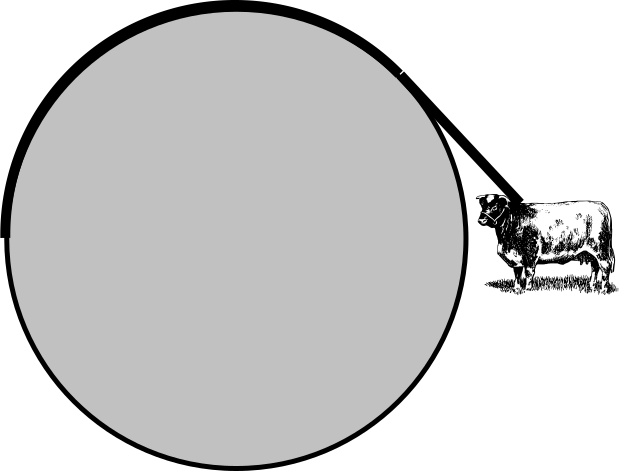
\includegraphics[width=0.9\columnwidth]{cowpic}
\end{center}

\end{multicols}


\newpage
%\thispagestyle{empty}





 \begin{enumerate}
\item Eliminate the parameter to obtain an equation for the curve involving only $x$ and $y$:
\begin{enumerate}
 \item $x=\sec t$, $y=\tan t$
 \item $x=4\sin t+1$, $y=3\cos t-2$ (Hint: first solve for $\cos t$ and $\sin t$.)
 \item $x=\dfrac{1}{t+1}$, $y=\dfrac{3t+5}{t+1}$. (Hint: try doing long division on the expression for $y$.)

\end{enumerate}

\vspace{3.5in}

\item Find any points of self-intersection for the following curves:
\begin{enumerate}
\item $x=t^3-t-3, y=t^2-3$
\item $x=\cos(t), y=\sin(2t), t\in [0,2\pi]$
\end{enumerate}

\newpage

 \item Find the length of the parametric curve:
\begin{enumerate}
 \item $x=-3\sin(2t)$, $y=3\cos(2t)$, $t\in [0,\pi]$.
 \item $x=e^{t/10}\cos t, y=e^{t/10}\sin t$, $t\in [0,2\pi]$.
\end{enumerate}

\vspace{4in}

 \item Find the area enclosed by the loop of the ``teardrop'' curve $x=t(t^2-1), y=t^2-1$. (See Figure 10.34 in the text.)


\newpage

\item For each curve below, find the equation of the tangent line at the given value of $t$. Also: find all points where the tangent line is horizontal or vertical.
\begin{enumerate}
\item $x=t^2-1$, $y=t^3-t$, $t=1$.

\vspace{3.5in}

\item $x=\cos(t), y=\sin(2t), t=\pi/4$
\end{enumerate}
\end{enumerate}
\end{document}